%!TEX root = paper.tex

Rather than looking at the explicit representation equation of lines in the plane, we can gain much more insight from looking at the parametric representation. To simplify our analysis, we will choose our time parameter such that v collisions occur every $\Delta t = 1$ and h collisions occur every $\Delta t = m$. The equation for a line $y(x) = m \, x + y_0$ is equivalent to the following parametric system

\begin{align}\label{eq:parametric-line}
	x(t)& = \frac{1}{m} \, t\\
	y(t)& = t + y_0
\end{align}

Now v and h collisions in the 2-dimensional plane can be projected onto the 1-dimensional $t$ axis as is shown in Figure \ref{fig:1d-projection}. 

\begin{figure}[H]
  \begin{center}
    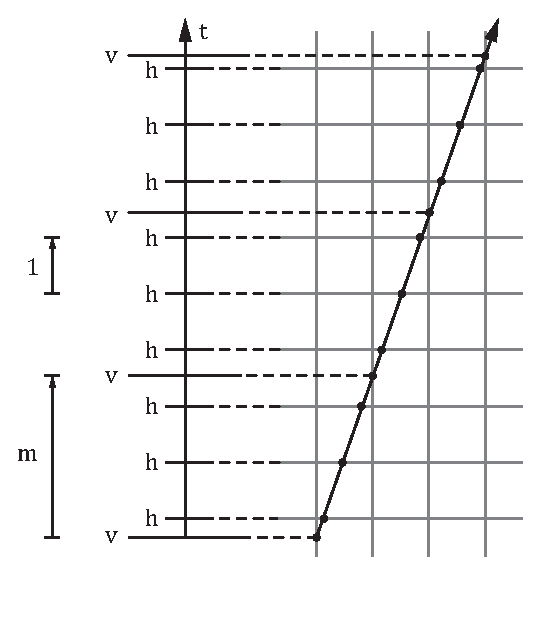
\includegraphics[keepaspectratio, height=4in]{1d_mapping_1}
  \end{center}
  \vspace{-.2in} % corrects bad spacing
  \caption{\label{fig:1d-projection} Projecting onto the $t$ axis.}
\end{figure}

For the sake of space, we will rotate the $t$ axis so that it is horizontal, as is shown in Figure \ref{fig:1d-problem}. The problem of mapping collision sequences to lines in the plane becomes a problem of fitting regularly spaced tick marks into intervals on the real number line.

\begin{figure}[H]
  \begin{center}
    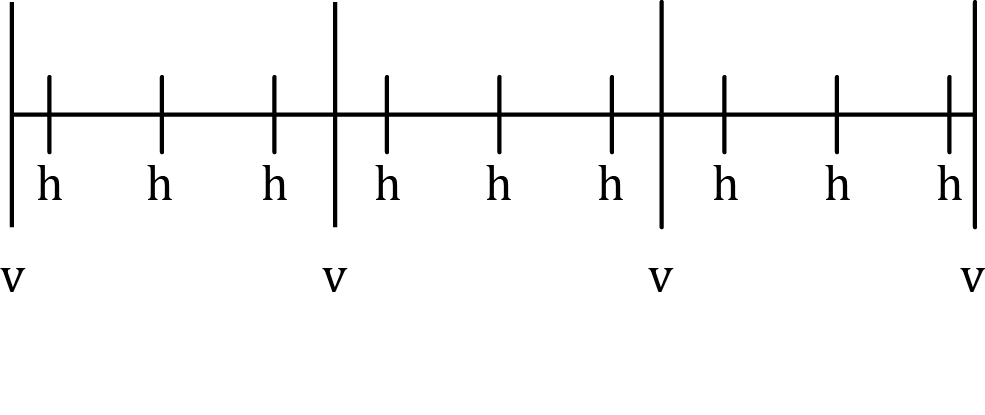
\includegraphics[keepaspectratio]{1d_mapping_2}
  \end{center}
  \vspace{-.2in} % corrects bad spacing
  \caption{\label{fig:1d-problem} The 1-dimensional problem.}
\end{figure}

% -----------------------------------------------------------------------------

To start off analyzing this 1-dimensional problem, we need a basic lemma about counting ticks marks inside an interval.

\begin{lemma}\label{lem:interval-ticks}
	Let $l_2 < l_1$. The number of real numbers at regular spacing $l_2$ inside an open interval of length $l_1$ is in $\cbracket{\floor{\frac{l_1}{l_2}}, \ceil{\frac{l_1}{l_2}}}$.
\end{lemma}

\begin{proof}
	Let $A \subset \Z$ represent the set of all possible numbers of real numbers at regular spacing $l_2$ inside an open interval of length $l_1$. Given some $a \in A$, let $b \in \R$ be defined such that the following holds

	\begin{equation}\label{eq:interval-ticks}
		l_1 = (a - 1) l_2 + b
	\end{equation}

	We know that $(a - 1) l_2 < l_1$, so $b \ge 0$. Also, $b < 2 \, l_2$, because otherwise, there must be more than $a$ real numbers inside the interval, contradicting our original assumption.

	Rearranging Equation \ref{eq:interval-ticks}, we get

	\begin{gather}
		a = \frac{l_1}{l_2} + 1 - \frac{b}{l_2}\\
		\frac{l_1}{l_2} - 1 < a < \frac{l_1}{l_2} + 1\\
		a \in \cbracket{\floor{\frac{l_1}{l_2}}, \ceil{\frac{l_1}{l_2}}}
	\end{gather}
\end{proof}
